\section{Electron Beam Melting: Finite Element Model}
\label{sec:model}

Electron beam melting (EBM) is an additive manufacturing process of fusing powder particles, layer-upon-layer, 
using an electron beam as the energy source. The process is typically used in the case of metals and its alloys.
Multiple passes of  a low power electron beam is used for heating and sintering the powder bed prior to selective
melting. For the application problem in this study, we focus on the thermo-mechanical behavior of an AM part
produced by the EBM process. For this purpose, we have developed a finite element-based thermal analysis
model to simulate the thermal response of the part and a finite element-based mechanical model that uses
the part's thermal
response to estimate the residual stress in the part at the end of the cooling phase. In this study, the two models are
weakly coupled i.e. the temperature history of the part is used as an input heat load for the mechanical model. 
Finite element analysis is performed using Abaqus~\cite{Hibbitt:2001}, a commercially available software. 

Our analysis is based on stress development in an AM part as a result of a single scan of an 
electron beam along its
length. A layer thickness, 50~$\mu$m and a part of dimensions (in mm), 2$\times 1.5\times 0.65$ is used as shown
in Figure~\ref{fig:PartwMesh}~(left). 
The process of laying the new powder on bulk material formed by previous scans is simulated 
by activating the initially deactivated elements representing the powder layer. To mitigate computational cost
associated with FEA, a non-uniform mesh is employed wherein a finer mesh is considered for the powder
region where the heat flux is applied. A gradually coarsening mesh is considered for the bulk material, significantly far 
from the heat source as shown in Figure~\ref{fig:PartwMesh}~(right). The mesh consists of 13,200 nodes and 
10,752 elements in total. 
%
\begin{figure}[htbp]
\begin{center}
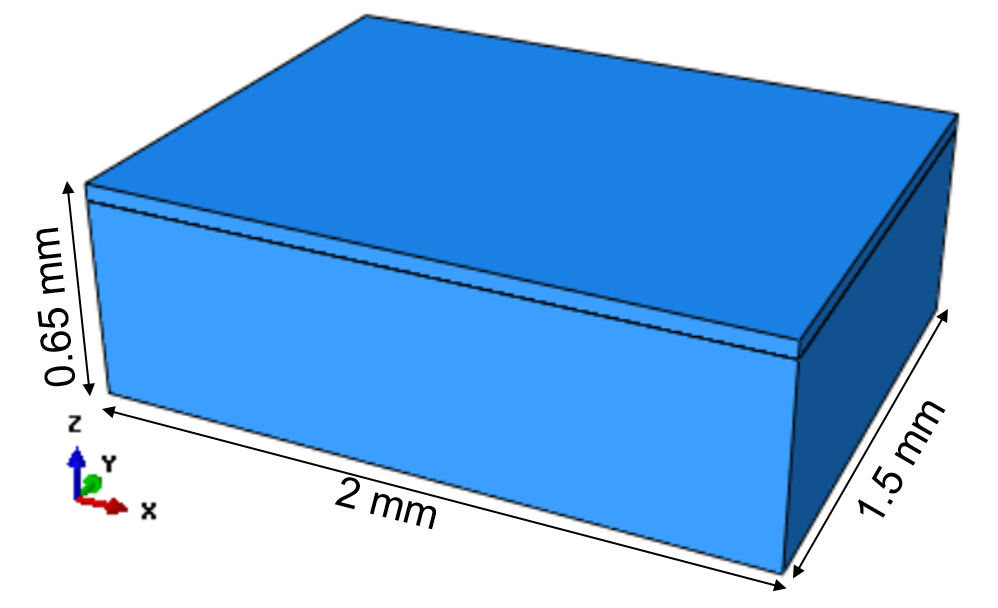
\includegraphics[width=0.4\textwidth]{./Figures/EBM_PartwXYZ} 
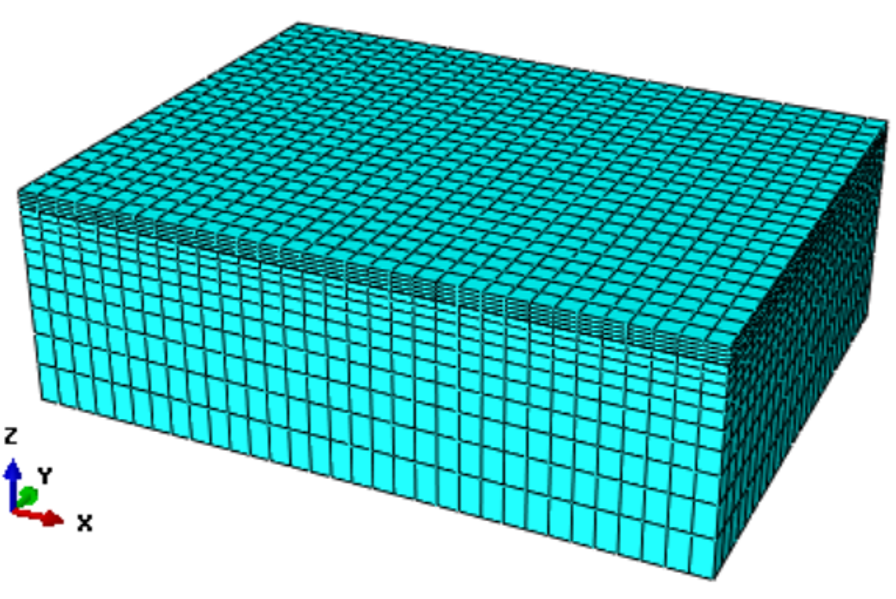
\includegraphics[width=0.4\textwidth]{./Figures/meshwXYZ}
\end{center}
\caption{Part geometry and the corresponding mesh as modeled in Abaqus}
\label{fig:PartwMesh}
\end{figure}
%
The material used to manufacture the part is considered to be Ti-6Al-4V and its
thermophysical properties considered in the finite element analysis are provided in Table~\ref{tab:matProp}.
%
\begin{table}[htbp]
\centering
\caption{Thermophysical properties of Ti-6Al-4V~\cite{Fu:2014}}
\label{tab:matProp}
\vspace{1mm}
\begin{tabular}{ ll }
\toprule
    Density (kg $/$m$^3$) & 4428\\
    Solidus Temperature ($^\circ$ C) & 1605 \\
    Liquidus Temperature ($^\circ$ C) & 1655\\
    Latent heat (J$/$kg) & 365000\\
    Elastic Modulus (GPa) & 110 \\
    Poisson's ratio & 0.41\\
    Yield strength (MPa) & 825\\
\bottomrule
\end{tabular}
\end{table}
%%%

\subsection{Thermal Model}
\label{sub:thermal}

The governing equation for the heat transfer analysis \cite{Zinoviev:2016} is given by:
\begin{equation}\label{eq_thermal}
\rho {C_p}\frac{{\partial T}}{{\partial t}} = -\nabla\cdot ({\kappa}\nabla T) + Q_e - Q_r 
\end{equation}
where $T$, $\rho$, $C_p$, $\kappa$, $Q_e$ denote the local temperature, average density, specific heat,  thermal 
conductivity, 
and the applied heat flux respectively. A single scan is considered along the x-direction at the top surface of the part. 
Heat flux due to the moving electron beam is modeled as a Gaussian~\cite{Vastola:2016} according to the following
equation:
%
\begin{equation}\label{eq_heatFlux}
Q_e = \frac{2P}{\pi r^2 d}\frac{1}{5}\Big[-3\Big(\frac{z}{d}\Big)^2-2\frac{z}{d}+5\Big]\exp\left({\frac{-2((x-vt)^2+y^2)}{r^2}}\right)
\end{equation}
%
where $P=\alpha IV$ denotes the power associated with the electron beam for a given absorptivity~($\alpha$),
current~(I), and voltage~(V). The quantities: $v$, $r$, and $d$ denote  the beam velocity or scan speed,
beam spot radius, and penetration depth respectively. The external heat flux is illustrated using temperature
contours on the top surface in Figure~\ref{fig:thermal}~(left) and along x-z plane passing through the center of the part in
Figure~\ref{fig:thermal}~(right). 
%
\begin{figure}[htbp]
\begin{center}
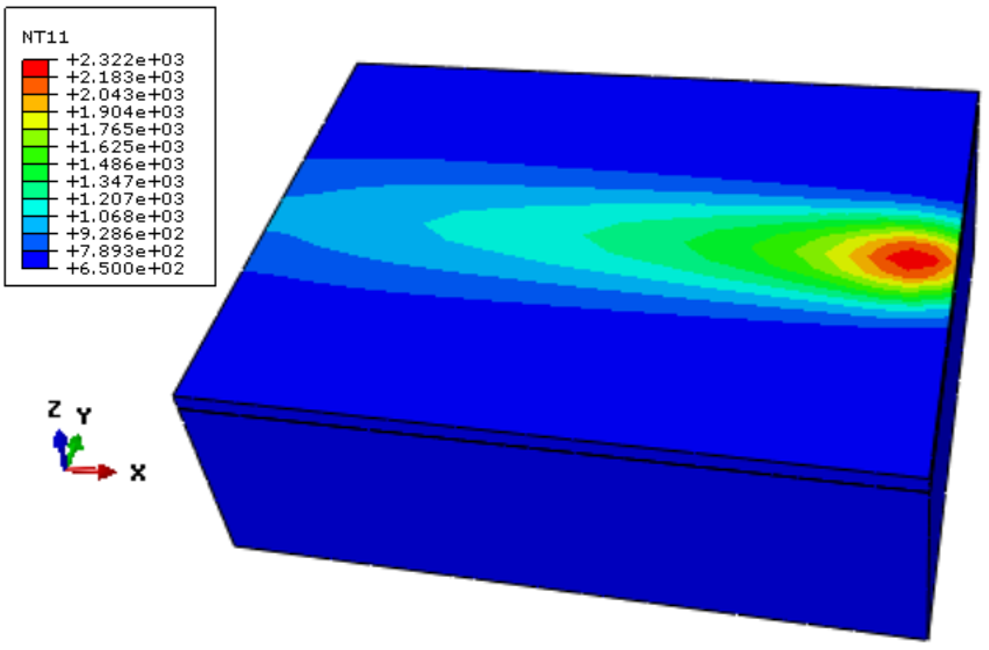
\includegraphics[width=0.42\textwidth]{./Figures/NT11Nom3D} 
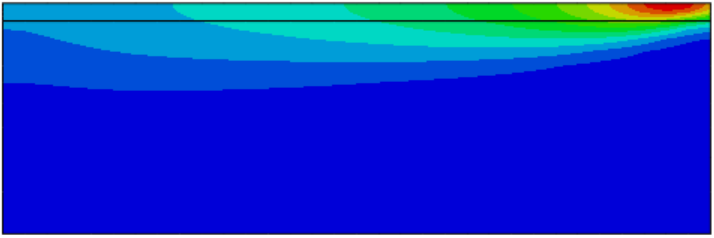
\includegraphics[width=0.42\textwidth]{./Figures/NT11Nom} 
\end{center}
\caption{Left: Temperature contours associated with the moving electron beam as a heat source. Right:
Temperature contours in the x-z plane passing through the center of the part once the electron beam is 
turned off.}
\label{fig:thermal}
\end{figure}
%

The laser beam radius~($r$) and the thermal penetration depth are fixed at 200 and 28
microns respectively. The powder is pre-heated to a temperature, $T_0$ prior to the scan using fixed temperature
boundary conditions at the lateral sides as well as the bottom of the part. Heat transfer in the part occurs by two
mechanisms: First, by means of thermal conduction due to temperature gradients especially along the depth (x-z plane),
and second, by means of radiative losses from the exposed surface of the part denoted as $Q_r$ in~\eqref{eq_thermal}.
The radiative heat flux, $Q_r$ is modeled using the Stefan-Boltzmann law i.e., $Q_r=\sigma\epsilon(T^4-T_a^4)$, where
$\sigma$, $\epsilon$, and $T_a$ denote the Stefan-Boltzmann constant, emissivity of the top surface, and the ambient
temperature respectively. Note that convective losses are not considered since the manufacturing process is 
assumed to be
carried out in vacuum. As discussed later in Section~\ref{sec:results}, the beam power~($P$), scan speed~($v$), and 
pre-heat temperature of the powder bed~($\theta_0$) are considered as process control parameters~($\bm{\theta_p}$)
in our analysis using the surrogate model. The temperature history of the part determined using the thermal model
is used as an input to the mechanical model (one way coupling) to compute residual stress in the AM part as 
discussed in the following section. 

\subsection{Mechanical Model}
\label{sub:mech}

The governing equation for structural analysis \cite{Megahed:2016} is given by:
%
\begin{equation}\label{eq_mechanical}
\nabla \cdot \mat{\sigma}+f = 0
\end{equation}
%
where $\sigma$ and $f$ denote the stress tensor and the internal forces respectively. From Hooke's law, the stress
tensor ($\mat{\sigma}$) is proportional to the total strain~($\epsilon^T$). Material stiffness tensor, $\mat{C}$ is the
proportionality constant. The constitutive relationship is given as follows:
%
\be
\mat{\sigma} = \mat{C}\epsilon^T
\ee
%
where $\epsilon^T = \epsilon^e + \epsilon^p+ \epsilon^t$; $\epsilon^e$, $\epsilon^p$, and $\epsilon^t$ denote elastic, 
plastic, and thermal strains respectively. The plastic strain is modeled by considering elastic 
perfectly-plastic~\cite{Zhao:2015} condition in the model. Thermal strain is calculated  from the thermal expansion 
constitutive relationship: $\varepsilon^T = \alpha_{t}\Delta T$, where $\alpha_t $ is the thermal expansion coefficient.
The boundary surfaces in the X-direction and Y-direction are constrained in the x-
coordinates and y-coordinates respectively. The bottom surface is considered fixed in all coordinates.
Temperature history at each node, obtained using the thermal model in~\ref{sub:thermal}, is used to
compute the strain tensor, $\sigma$. Hence, the mechanical model is dependent on the thermal response
of the part but not vice versa. The coupling between the two model is therefore regarded as \textit{one-way}
or \textit{weak}~\cite{Debroy:2017}. Weak coupling between the models is essentially considered due to the fact
that a strong coupling would be computationally expensive. The von Mises stress at the end of the cooling process
is considered as the residual stress in the AM part~\cite{Vastola:2016}. 
It is considered as the quantity of interest~(QoI) in our analysis for 
demonstrating the methodology proposed earlier in Section~\ref{sec:method}. The stress contours are illustrated
in Figure~\ref{fig:subSmises} 
%
\begin{figure}[htbp]
\begin{center}
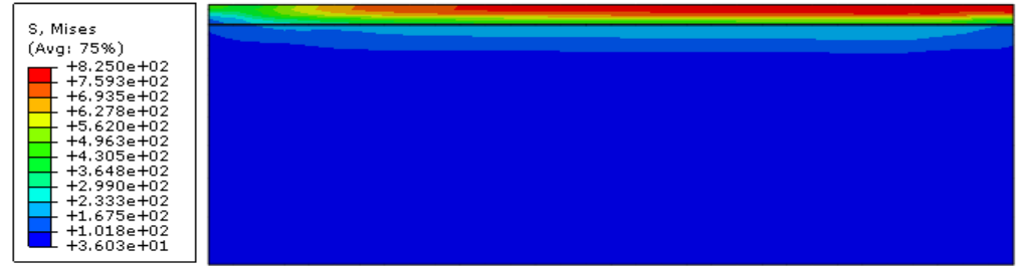
\includegraphics[width=0.6\textwidth]{./Figures/SMisesNom} 
\end{center}
\caption{von Mises stress contours in the x-z plane passing through the center of the part after it has cooled
down to the ambient temperature.}
\label{fig:subSmises}
\end{figure}
%
The contour plot in Figure~\ref{fig:subSmises} clearly indicates that the residual stress in the part attains higher
values near the top surface and diminishes quickly along the depth of the part. It can thus be said that thermal
strain due to the applied heat flux is the dominant contributor to the residual stress in the present set-up. 

Simulations are performed on a workstation with a system configuration: Intel~Core~i7-4790~CPU, 
3.60 GHz with 16GB RAM. It is observed that on average the thermal model takes 20 minutes to complete 
a run, and the
mechanical model takes 10 minutes. Note, however, that the simulation duration depends on the choice of
values for the set of inputs.  


























